% ######################################################################
%
% 			PREAMBULE
%
% ######################################################################

% -------------------------------------------------------
% Ce document est un raport. dizaine de pages / plusieurs sections
% -------------------------------------------------------
\documentclass[a4paper,12pt]{report}

% -------------------------------------------------------
% Utiliser latin1 pour les accents
% ne pas utiliser utf8 et Latex n'aime pas utf8 ET latin1
%\usepackage[utf8]{inputenc}
% -------------------------------------------------------
\usepackage[utf8]{inputenc}

% Vu dans un forum : utiliser plutôt frenchb, french est obsolete
\usepackage[T1]{fontenc}
\usepackage[english,frenchb]{babel}

% -------------------------------------------------------
% Trouvé dans un forum a voir plus tard
% utile ou pas
% significations
% -------------------------------------------------------
\usepackage{amsmath}
\usepackage{amssymb,amsfonts,textcomp}
\usepackage{color}
\usepackage{array}
\usepackage{supertabular}
\usepackage{hhline}
\usepackage{hyperref}
\usepackage{lmodern}
\usepackage{xspace}
% \usepackage{unicode-math}	% pour prime dprime tprime

% -------------------------------------------------------
% Théorèmes
% -------------------------------------------------------
\usepackage{amsthm}
\theoremstyle{plain}				% Choix du style
\newtheorem{theoreme1}{Théorème}	% Définition de l'environnement 1

\theoremstyle{definition}				% Choix du style
\newtheorem{definition1}{Definition} %[section]	% Définition de l'environnement définition
% -------------------------------------------------------
%pour utiliser
% \textsubscript{}
% {\textbar}
% -------------------------------------------------------
\usepackage{fixltx2e}

% -------------------------------------------------------
%BIBTEX
% -------------------------------------------------------
\usepackage{natbib}

%____________________________________________________________________
%
% Tout ceci ne fonctionne pas ! ou n'ai pas réussi à faire fonctionner
% \usepackage[backend=bibtex, style=numeric]{biblatex}	% Compilateur
% \bibliography{Bibliographie}			% Utilise Bibliographie.bib
% \addbibresource{Bibliographie.bib}
% \bibliographystyle{plain}
%____________________________________________________________________

% -------------------------------------------------------
% Pour les tableaux
% -------------------------------------------------------
%\usepackage{slashbox}
\usepackage{diagbox} % barre oblique pour les cellule à 2 entrées


% -------------------------------------------------------
% Pour les ALGORITHMES
% linesnumbered	: les lignes sont numérotées
% ruled			: Le caption est en haut et bordé de lignes horizontale
% vlined		: Regroupement des bloc d'instructions par ligne verticales
% -------------------------------------------------------
\usepackage[linesnumbered, ruled, vlined]{algorithm2e}
\SetKwProg{Init}{init}{}{}
% mettre les commentaire des algos en bleu
\usepackage{xcolor}
\newcommand\commentairesBleus[1]{\footnotesize\ttfamily\textcolor{blue}{#1}}
\SetCommentSty{commentairesBleus}

% -------------------------------------------------------
% Information PDF généré
% -------------------------------------------------------
\hypersetup{pdftex, colorlinks=true, linkcolor=blue, citecolor=blue, filecolor=blue, urlcolor=blue, pdftitle=, pdfauthor=florianColas, pdfsubject=, pdfkeywords=}
\usepackage[pdftex]{graphicx}

\newcommand\PCmax{$P||C_{\max}$\xspace}
\newcommand\PmCmax{$P_m||C_{\max}$\xspace}

% Ajout L. Philippe
\usepackage{todonotes}
\newcommand{\tdi}[1]{\todo[inline]{{#1}}{}}
\newcommand{\lp}[1]{\todo[author=LP,inline]{#1}}
\newcommand{\lcc}[1]{\todo[author=LCC,color=green,inline]{#1}}

% -------------------------------------------------------
% Information générales
% Utilisé par \maketitle
% -------------------------------------------------------
\title{Historique des travaux autour du problème P{\textbar}{\textbar}Cmax}
\author{florian colas}
% \date{2020-05-01}
\date{\today}


% ######################################################################
%
% 			SOUVENT UTILISES
%
% ######################################################################
% Pm||Cmax 				: \PmCmax
% P2||Cmax 				: P\textsubscript{2}{\textbar}{\textbar}C\textsubscript{max}
% P||Cmax 				: P{\textbar}{\textbar}C\textsubscript{max}
%
% Appostrophes 			: '
%
% en italique car latin : \textit{et al.}
%
% entourer un résultat
%	\begin{center}
%	\fbox{\begin{minipage}{\linewidth}
%	bla blabla
%	\end{minipage}}
%	\end{center}


% ######################################################################
%
% 				DOCUMENT
%
% ######################################################################

\begin{document}

% =======================================================
% Page de garde
% Utilise Information générales
% Ecrit le titre + auteur + date
% =======================================================
\maketitle

% -------------------------------------------------------
% Table des matières
%
% On renomme en Sommaire (document français)
%
% On définit la profondeur de la table des matières
% -1 partie,    0 Chapitre,
% 1 Section,    2 sous sections,  3 sous sous section
% 4 Paragraphe, 5 Sous paragraphe
%
% Les sections sont numérotées 1 2 3
% -------------------------------------------------------
\renewcommand{\thesection}{\arabic{section}}
\renewcommand{\contentsname}{Sommaire}
\setcounter{tocdepth}{4}	% avant 2pour la table des matières
\setcounter{secnumdepth}{3}	% pour les section sous et sous sous et paragraphes
\tableofcontents

% =======================================================
% 1 INTRODUCTION
% =======================================================
\section{Introduction}

texte


\section{Présentation du problème.}
texte
\subsection{Parallélisme.}
Le parallélisme est un type d{\textquotesingle}architecture informatique
dans lequel plusieurs processeurs exécutent ou traitent une application
ou un calcul simultanément. Il aide à effectuer de grands calculs en
divisant la charge de travail entre plusieurs processeurs, qui
fonctionnent tous en même temps.

Il existe quatre types de parallélismes, définis par la taxonomie de
Flynn\textsuperscript{(1)}. Cette classification est basée sur deux
notions: le flot d'instructions (simple ou multiple),
et le flot de données (simple ou multiples); un algorithme est un flot
d'instructions à exécuter sur un flot de données.

\lp{la classification de Flynn date un peu... Peut-être faut-il
  trouver qlqchose de plus récent}

% -------------------------------------------------------
% TABLEAU taxonomie de Flynn
% diagbox permet d'avoir une barre oblique pour les deux entrées
% \backslashbox{Instructions}{Donnée} & Simple & Multiple NE FONCTIONNE PAS
% on cadre à gauche le tableau pour avoir plus de place
% -------------------------------------------------------
\begin{flushleft}
\begin{tabular}{|p{3.6cm}|p{6cm}|p{6cm}|}

% --------------------------
% TITRES
% --------------------------
\hline
\diagbox[width=10em]{Instructions}{Données} & Simple & Multiple \\
\hline

% --------------------------
% LIGNE SIMPLE
% --------------------------
Simple

%---------------------------
&
SISD

premiers PC

machine de Von Neumann

~

Obsolète, car tous les PC sont désormais multi-c{\oe}ur.
%---------------------------
&
SIMD

Machines synchrones

Pipeline

~

Exécution d'une instruction unique sur des données différentes.
\\	\hline
% --------------------------
% LIGNE MULTIPLE
% --------------------------

Multiple

%---------------------------
&
MISD

Machines vectoriels

Tableau de processeurs

~

Exécute plusieurs instructions sur une même donnée.
%---------------------------
&
MIMD

Multi processeurs à mémoire distribuée.

Multi processeurs à mémoire partagée (multi-c{\oe}ur).

Multi Ordinateur.
%---------------------------
\\
\hline
\end{tabular}
Taxonomie de Flynn
\end{flushleft}


Les premières machines parallèles étaient des réseaux
d'ordinateurs, et des machines vectorielles (faiblement
parallèles, très coûteuses), telles que l'IBM 360, les
Cray1. La plupart des machines parallèles contemporaines sont désormais
MIMD.
\lp{Ce n'est pas si simple. On continue de faire, et d'utiliser
  des machines vectorielles, les GPU sont aussi du SIMD...}

On peut définir une machine parallèle comme un ensemble de processeurs
qui coopèrent et communiquent.

\bigskip

\begin{figure}
\centering
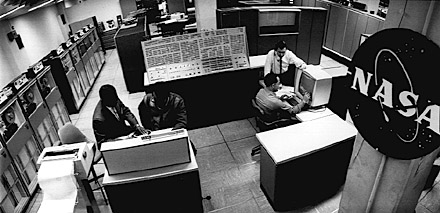
\includegraphics[width=8.334cm,height=4.034cm]{Biblio_PCmax_Rendu-img1.jpg}
\caption{
IBM 360-91 (le plus rapide et le plus puissant en service en 1968) NASA.
Centre de vols de Greenbelt (Md)
}
\end{figure}

\lp{pense à compléter cette partie avec des infos sur des
  machines actuelles. voir top500.org dont il serait peut-être plus
  judicieux de citer les infos: puissance des plus gros ordinateurs,
  nombre de proc, cores, etc. Parler peut-être aussi des clouds ? Des
  applications ? Pour intro}


\subsection{Ordonnancement}

Sur une machine non parallèle, les tâches sont exécutées
séquentiellement, les unes après les autres.
Certaines tâches, ou jobs peuvent demander plus de temps que d'autres
pour être entièrement traitées.
Lorsque plusieurs ressources (processeurs, machines, coeurs) sont
disponibles, ou que des jobs a exécuter ne sont pas indépendants (même
traités sur un seul processeur), se pose alors, un problème
d'ordonnancement.
Celui-ci consiste à organiser, dans le temps, les jobs à exécuter, en
les affectant à une ressource donnée, de manière à satisfaire un
certain nombre de contraintes, tout en optimisant un ou des objectifs.
L'ordonnancement fait partie de la catégorie des problèmes
d'optimisation combinatoire.

Les problèmes qui s'y rattachent sont très variés.
Premièrement, la nature des machines parallèles doit être considérée.
Celles-ci peuvent être:
\begin{description}
\item[identiques] le même temps de traitement sera nécessaire, d'une
  machine à l'autre;
\item[uniformes] un quotient de vitesse $q_i$ propre à une machine est à
  appliquer pour chaque tâche affectée à cette machine pour déterminer
  le temps de traitement nécessaire;
\item[indépendantes] les temps de traitements des tâches sont ni
  uniformes ni proportionnels d'une machine à l'autre.
\end{description}
Ensuite, des contraintes peuvent affecter les jobs eux-mêmes.
Dans le cas d'un problème préemptif, les taches peuvent être
interrompues, et reprises ultérieurement.
Il est possible que les jobs soient indépendants, ou au contraire,
être liées par des relations de précédence.
Ces jobs ne sont disponibles qu'à partir d'une certaine date.
Ou encore, être de durée égale, ou tous de durée différente.

Pour finir, l'objectif de
l'ordonnancement est d'optimiser un
critère. Par exemple, minimiser la somme des dates de fin, la somme
des retards, le nombre de tâches en retard, ou simplement, le retard
total. Mais le plus habituel, est de chercher à minimiser le temps
total de traitement de tous les jobs, i.e minimiser le makespan.

\lp{définir la notation de Graham à la fin de cette partie
  puisque tout y est déjà dit.}


\subsection{Enoncé du \PCmax}

Ces diverses possibilités définissent divers problèmes
d'ordonnancements différents, recensés et classifiés
\ par Graham et al. [1], qui introduit la notation trois-champs $\alpha
${\textbar}$\beta ${\textbar}$\gamma $ .

\bigskip

Le problème \PmCmax se définit alors ainsi:

\begin{itemize}

% -------------------------------------------------------
% ALPHA P Type de machines
% -------------------------------------------------------
\item $\alpha = \alpha_1 \alpha_2$, détermine l'environnement
  machines.
  $\alpha P$: les machines sont parallèles et identiques: un job,
  une tâche prendra le même temps de traitement qu'il soit exécuté sur
  une machine ou une autre.
  Le nombre de machines ($m$) est variable.

% -------------------------------------------------------
% BETA Contraintes
% -------------------------------------------------------
\item $\beta \subset \{ \beta_1, \beta_2, \beta_3,
  \beta_4, \beta_5, \beta_6\}$, détermine les caractéristiques
  des jobs, ou des tâches.
  $\beta $ est vide.
  Ce qui signifie que la préemption n'est pas autorisée (les jobs
  doivent être exécutés d'une traite, sans interruption ni coupure) \
  et qu'il n'y a pas de relation entre les jobs (ils sont
  indépendants).

% -------------------------------------------------------
% GEMEL Optimisation
% -------------------------------------------------------
\item $\gamma $ détermine le critère à optimiser.
$\gamma C_{\max}$: on cherche à optimiser le makespan,
i.e.\ le temps de traitement total.

\end{itemize}

\bigskip

\begin{definition1}{\PmCmax}
  \PmCmax consiste à planifier un ensemble $J = \{1,2,\ldots,\}$
  de n jobs simultanés, pour être traités par m machines identiques et
  parallèles.
  Chaque job, qui requière une opération, peut être traité par une des
  m machines.
  Le temps de traitement de chaque job (P\textsubscript{i} avec
  i~${\in}$ N) est connu à l'avance.
  Un job commencé, et complété sans interruption.
  Les jobs, indépendants, sont exécutés par une seule machine, et une
  machine ne peut traiter qu'un seul job à la fois.

\end{definition1}

\lp{on peut recontextualiser l'intérêt du problème. A l'heure
  actuelle, bon nombre de centres de calcul ont un parc
  assez homogène. De même les clouds offrent des instances de VM, ce
  qui permet d'avoir un environnement d'exec homogène }

\lp{faire un dessin illustratif ?}

\lp{dire que la difficulté repose uniquement sur le regourpement
  des jobs sur une machine puisque les machines sont identiques}

\subsection{Problématique}

Comme l'ont démontré Garey et Johnson, $P_2||C_{\max}$ est un
problème NP-Difficile \cite{garey1978strong}, et \PCmax est un
problème NP-Difficile au sens fort \cite{garey1982computers}.
Cependant, \PmCmax devient un problème NP-Difficile, du moment que le
nombre de machines est fixé \cite{chen1999potts}, comme l'a montré
Rothkopf \cite{rothkopf1966scheduling}, qui a présenté un algorithme
de programmation dynamique.

Donner la solution optimale à un problème d'ordonnancement (dans notre
cas \PmCmax) n'est pas réaliste.
Même pour un problème de taille modeste, la résolution de celui-ci
demanderait un temps excessif et donc rédhibitoire.

La résolution du problème d'ordonnancement va reposer sur des méthodes
d'approche\todo{LP: approximation?}, qui consistent à calculer en
temps polynomial, une solution ``assez'' proche de la valeur optimale.

Dans la littérature, l'étude d'ordonnancement est très riche et
abondante.
Le but étant d'améliorer le temps de calcul, et d'approcher le
résultat optimal.

\section{Résoudre le problème}

Comme évoqué précédemment, l'existence d'une solution qui résout le
problème n'est pas pensable, à moins que $P = NP$.

\subsection{Notations utilisées}

Chaque document utilise sa propre notation, mais les notions sont les mêmes.
Soient les données du problème

\begin{itemize}
% -------------------------------------------------------
% ENSEMBLE DES JOBS J
% -------------------------------------------------------
\item un ensemble de $n$ jobs (ou tâches) $J = \{1, 2, ..., n\}$.
  Chaque job $j$ a un temps de traitement connu $p_j$
  ($P = \{p_{1}, p_{2}, \ldots, p_{n}\}$).

% -------------------------------------------------------
% ENSEMBLE DES MACHINES M
% -------------------------------------------------------
\item $m$ machines parallèles identiques $M_i$ avec ($i =
  1, 2, \ldots, m$).

  \lp{au besoin définir $M = \{ m_1, m_2, \ldots, m_m \}$ mais du
  coup il faut choiir à quoi sert le $m$}

% -------------------------------------------------------
% RESULTAT DE L'ALGORITHME A
% -------------------------------------------------------
\item $C_j^A(J)$ le résultat de l'ordonnancement d'un ensemble $J$ de
  jobs, sur $m$ machines parallèles, identiques, obtenu par
  l'algorithme $A$.
  \lp{à quoi sert $j$ ici ?}

% -------------------------------------------------------
% RESULTAT OPTIMAL
% -------------------------------------------------------
\item $C_j^\star(J)$ le makespan optimal, idéal.
  \lp{idem}

% -------------------------------------------------------
% RATIO OBTENU/OPTIMAL
% -------------------------------------------------------
\item $\Gamma(A)=\dfrac{C_j^A(J)}{C_j^\star(J)}$ le ratio
  d'approximation atteint par l'algorithme A au pire
  cas.

  \lp{idem}
\end{itemize}

\subsection{Heuristiques}

\lp{définir heuristic ?}

Les heuristiques présentent plusieurs avantages. Leur complexité est
réduite\lp{ça dépend de leur conception}, et obtiennent de bonne
performances\lp{ça dépend aussi, je suis capable de faire des
heuristiques non performantes}. Elles représentent la plus grande
partie des recherches concernant le problème
d'ordonnancement, même si leurs performances, au pire
cas, ne sont pas\todo{LP: ??} garanties.
Sont abordées ici les heuristiques les plus présentes dans la littérature.

\lp{on a aussi une borne min qui est le max entre la plus grande
  des tâches et sum(pi)/m}
\subsubsection{Basé LS (List Scheduling)}
% '

L'idée d'une LS est de stocker l'ensemble des jobs dans celle-ci, les
trier dans un ordre particulier, avant de les affecter à une machine
selon des règles définies.

\lp{un algorithme de liste affecte aussi un job, le premier de la
liste, à la première machine prête}
%\bigskip
% -------------------------------------------------------
% LPT Rule
% -------------------------------------------------------
\paragraph{LPT rule (Graham \textit{et al.}, 1969)}

% Présentaion
% ---------------------
Graham propose \emph{Longest Processing Time (LPT) rule} \cite{graham1969bounds}.

\bigskip
% Algorithme
% ---------------------
\begin{algorithm}[H]
\DontPrintSemicolon
\KwData{instance de \PmCmax, avec m machines, n jobs et leur temps d'exécution}
%\Begin{ %inutile ici et rajoute un nuero de ligne

\BlankLine % Petit espace
Trie les jobs de l'ensemble $J$ dans l'ordre décroissant de leur temps
d'exécution et ré-indexe l'ensemble de telle manière à obtenir:
$p_1 \geq p_2 \geq ...
\geq p_n$

\BlankLine % Petit espace
Parcours la liste, et affecte chaque job à la machine la moins
chargée, à ce moment là.
% }
\caption{LPT Rule\label{LPT}}
\end{algorithm}

\bigskip
% Exemple
% ---------------------
Exemple

Soit $P=\{13,10,7,6,6,5,3,2\}$, l'ensemble des $p_j$ déjà triés dans
l'ordre décroissant à appliquer sur 4 machines parallèles identiques:

{\centering
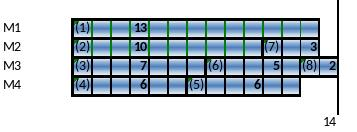
\includegraphics[width=8.334cm,height=4.034cm]{Biblio_PCmax_Rendu_exLPT1.jpg}
\par}
{\centering
\par}
Nous obtenons $C_4^{LPT}(J)=14$

\bigskip

% Complexité
% -------------------------------------------------------
\begin{flushleft}
\begin{tabular}{|p{10cm}p{4cm}|}
% TITRES (pas de titre)
\hline

% Ligne blanche
 & \\

% Ligne Complexité
Le tri puis l'affectation s'effectuent en & $O(n \log n + n \log m)$
\\	% pas de ligne \hline

% RATIO
Le ratio d'approximation	&	$\Gamma(LPT)\leq \dfrac{4}{3} - \dfrac{1}{3m}$
\\

% Ligne blanche
& \\
\hline
\end{tabular}
%pas de legende
\end{flushleft}

%\bigskip
% -------------------------------------------------------
% LPT-REV
% -------------------------------------------------------

\paragraph{LPT-REV (Croce \textit{et al.}, 2018)}

% Présentaion
% ---------------------
Le ratio d'approximation obtenu par LPT (\ref{LPT})
$(\Gamma(LPT)\leq \dfrac{4}{3} - \dfrac{1}{3m})$ est une borne
supérieure que cet algorithme peut atteindre, mais qu'il ne dépassera
jamais.
Chaque utilisation de LPT produira un résultat dont le ratio $\Gamma$
oscillera entre 1 et $\dfrac{4}{3} - \dfrac{1}{3m}$.

\bigskip
% Exemple pour l'explication
% ---------------------
Exemple de pire cas

Soit $P=\{7,7,6,6,5,5,4,4,4\}$, l'ensemble des $p_j$ déjà triés dans
l'ordre décroissant à appliquer sur 4 machines parallèles identiques:

\bigskip

% partie insécable
\begin{minipage}{\linewidth}

\begin{flushleft}
LPT donne le résultat suivant
\end{flushleft}
{\centering
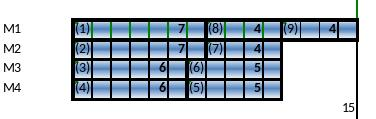
\includegraphics[width=8.334cm,height=4.034cm]{Biblio_PCmax_Rendu_exLPT_Rev1.jpg}
\par}

\begin{flushleft}
$C_4^{lpt}(J)=15$
\end{flushleft}

\end{minipage}

\bigskip

% partie insécable
\begin{minipage}{\linewidth}

\begin{flushleft}
Un ordonnancement optimal aurait été:
\end{flushleft}

{\centering
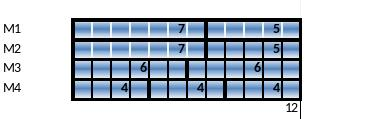
\includegraphics[width=8.334cm,height=4.034cm]{Biblio_PCmax_Rendu_exLPT_Rev2.jpg}
\par}


\begin{flushleft}
$C_4^{\star}(J)=12$
\end{flushleft}

\end{minipage}

Soit une marge de $\dfrac{15}{12}$

Le ratio d'approximation prévu pour $m=4$:
$\dfrac{4}{3} - \dfrac{1}{3m}=\dfrac{16}{12} - \dfrac{1}{12}=\dfrac{15}{12}$

Ce cas représente donc un pire cas pour LPT.

Croce \textit{et al.}
\cite{della2018longest}, en examinant le comportement de LPT rule,
notamment au niveau du ratio d'approximation, constatent que celui-ci
peut être réduit selon certaines configurations, ou instances du
problème, et rédigent le théorème suivant:

\bigskip

\begin{theoreme1}
  LPT a un rapport d'approximation non supérieur à
  $\dfrac{4}{3} - \dfrac{1}{3(m-1)}$ pour $m \geq 3$ et $n \neq 2m+1$.

  LPT atteint la limite de Graham $\dfrac{4}{3} - \dfrac{1}{3m}$ pour
  $m \geq 2$ et uniquement dans le cas où $n=2m+1$, et la machine
  critique traite 3 jobs, tandis que les autres en traitent 2.

  La machine critique est la machine qui exécute le job critique.

  Le job critique (noté $J^\prime$) est le job qui détermine le
  makespan.
\end{theoreme1}

\lcc{Les définitions à l'extérieur des théorèmes.}

\bigskip

Le rapport $\dfrac{4}{3} - \dfrac{1}{3(m-1)}$ est inférieur au
ration $\dfrac{4}{3} - \dfrac{1}{3m}$ (quel que soit le nombre de
machines)

\bigskip

NB

L'exemple précédant (pire cas) a les caractéristiques suivantes:
\begin{itemize}
	\item nombre de job $n=2m+1$.
	\item la machine critique exécute 3 jobs.
	\item les autres exécutent 2 jobs.
	\item un rapport d'approximation de $\dfrac{4}{3} - \dfrac{1}{3m}$
\end{itemize}

\bigskip

Une modification à l'algorithme LPT rule est apportée afin de placer
le problème \PmCmax toujours dans une instance où le ratio
d'approximation est $\leq \dfrac{4}{3} - \dfrac{1}{3(m-1)}$.
Cette modification consiste à planifier en premier, le job critique
sur une machine M1.

\bigskip

% Algorithme
% ---------------------
\begin{algorithm}[H]
\DontPrintSemicolon
\KwData{instance de \PmCmax, avec m machines, n jobs}
%\Begin{ %inutile ici et rajoute un nuero de ligne

Apply LPT yielding a schedule with makespan $z_1$ and $k-1$ jobs on
the critical macine before job $J^\prime$ \BlankLine % Petit espace
Apply $LPT^\prime = LPT(J^\prime)$ with solution value $z_2$

\BlankLine % Petit espace
\textbf{If} $m=2$ \textbf{then} apply
$LPT''=LPT([(J^\prime - k + 1), ...
, J^\prime])$ with solution value $z_3$ and \textbf{return}
$\min[z_1,z_2,z_3]$

\BlankLine % Petit espace
\textbf{Else} \textbf{return} $\min(z_1,z_2)$

\caption{LPT-Rev\label{LPTRev}}
\end{algorithm}


\bigskip

% Complexité
% -------------------------------------------------------
\begin{flushleft}
\begin{tabular}{|p{10cm}p{4cm}|}
% TITRES (pas de titre)
\hline

% Ligne blanche
 & \\


% RATIO
Le ratio d'approximation	&	$\Gamma(LPT-REV)\leq \dfrac{4}{3} - \dfrac{1}{3(m-1)}$
\\

% Ligne blanche
& \\
\hline
\end{tabular}
%pas de legende
\end{flushleft}


\subsubsection{Basé Bin-Packing}

Le problème Bin-packing, est semblable au problème \PmCmax.
Il consiste à ranger des objets de taille différentes, dans des bacs
identiques, tout en minimisant leur nombre.

L'ensemble des $n$ jobs $J = \{1, 2, ..., n\}$, et de leurs temps de
traitement $p_j P = \{p_1, p_2, ..., p_n\}$, peuvent être vus
respectivement comme:
\begin{itemize}
\item un ensemble d'objets $T = \{T_1, T_2, ..., T_n\}$
\item leur taille $L(T_i)$
\end{itemize}
Une taille maximale $C$ des bacs (ou boites) est donnée.
\bigskip

\begin{definition1}{Packing}
  Un packing, est une partition $P<P_1, P_2, ..., P_m>$ tel que
  $L(P_j) \leq C$ avec $1 \leq j\leq m$.
  Le but est de placer les objets $T_i$ dans des bacs $P_j$ de taille
  $C$, de manière à minimiser le nombre de bacs $m$.
\end{definition1}

L'idée est d'utiliser le problème Bin-Packing à l'envers, pour
approcher une solution au problème d'ordonnancement.

\lp{petite remarque sur la complexité du problème ?}


% -------------------------------------------------------
% MULTIFIT
% -------------------------------------------------------
\paragraph{MULTIFIT}

% Présentaion
% ---------------------
Coffman \textit{et al.} \cite{coffman1978application} se sont
intéressés à l'algorithme FFD (First Fit Decreasing), un outil de
résolution du problème de Bin-Packing, pour l'adapter au problème
\PCmax.
$FFD(T,C)$ renvoie le nombre de bacs de taille C non vides
nécessaires, et l'arrangement correspondant de l'ensemble $T$ d'objets.

\bigskip
% Principe de l'algorithme
% ---------------------
Soit $T_m^\star = \min\{C:FFD(T,C) \leq m\}$ la plus petite valeur de
$C$ (taille des bacs) qui permet à $T$ d'être pacqué dans $m$ (ou moins)
bacs.

\bigskip

Le but de MULTIFIT est donc de réduire la valeur de $C$, faire tourner
$FFD(T,C) $, jusqu'à ce que le nombre $m$ de bacs, alors devenu
insuffisant, augmente à $m+1$.
Cette valeur charnière de $C$ est $T_m^\star$, qui correspond au
makespan minimum recherché, de l'ordonnancement de l'ensemble $T$ de
jobs sur $m$ machine identiques parallèles.
\lp{deux mots pour dire comment est implémentée la recherche}


{\centering
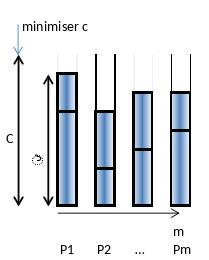
\includegraphics[width=6.138cm,height=7.62cm]{Biblio_PCmax_Rendu_exMULTIFIT1.jpg}
%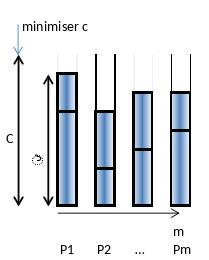
\includegraphics[width=8.334cm,height=4.034cm]{Biblio_PCmax_Rendu_exMULTIFIT1.jpg}

\par}
{\centering
Fonctionnement de FFD et principe de MULTIFIT
\par}

\bigskip

% Algorithme
% ---------------------
\begin{algorithm}[H]
\DontPrintSemicolon
\KwData{T un ensemble de jobs

m, un nombre de processeurs

borne supérieure: $Cu[T,m] = \max\{\dfrac{2}{m} \cdot L(T), \max_i\{L(T_i)\} \}$

borne inférieure: $Cl[T,m] = \max\{\dfrac{1}{m} \cdot L(T), \max_i\{L(T_i)\} \}$

k un nombre d'itérations
}

\BlankLine % Petit espace
La recherche de $T_m^\star$ s'effectue par dichotomie sur k itérations

\BlankLine % Petit espace
Après les k itérations, MULTIFIT \textbf{ renvoie $Cu(k)$} qui
correspond à la plus petite valeur de $C$ pour laquelle $FFD[T,C] \leq
m$

\lp{$k$ fixé ? ou seuil entre deux iter ?}

\caption{MULTIFIT\label{MULTIFIT}}
\end{algorithm}

\bigskip

% Complexité
% -------------------------------------------------------
\begin{flushleft}
\begin{tabular}{|p{10cm}p{4cm}|}
% TITRES (pas de titre)
\hline

% Ligne blanche
 & \\

% Ligne Complexité
Tri puis k FFD s'effectuent en & $O(n \log n + kn \log m)$
\\	% pas de ligne \hline

% Ligne blanche
 & \\

% RATIO
Ratio \cite{lee1988multiprocessor} & $\Gamma(MULTIFIT) \leq 1,220 + 2^{-k}$

\\

% Ligne blanche
& \\
\hline
\end{tabular}
%pas de legende
\end{flushleft}

Généralement, MULTIFIT donne des résultats très satisfaisant avec $k = 7$


% -------------------------------------------------------
% COMBINE
% -------------------------------------------------------
\paragraph{COMBINE}

% Présentaion
% ---------------------
Lee \textit{et al.}, \cite{lee1988multiprocessor} ont l'idée
d'utiliser LPT (\ref{LPT}) pour réduire les bornes de départ de
MULTIFIT (\ref{MULTIFIT}) dans un algorithme nommé COMBINE.

\lp{développer/préciser un peu}
\bigskip
soient
\begin{align*}
&la moyenne des poids des jobs par processeur &A &= \sum_{i=1}^{n}(\dfrac{P_i}{m})\\
&et &M &= C_m^lpt(J) \\
& &M^\star &= C_m^\star(J)
\end{align*}
 Si $M \geq 1,5\cdot A$ alors $M^\star = M$

\bigskip

% Algorithme
% ---------------------
\begin{algorithm}[H]
\DontPrintSemicolon
\KwData{instance de \PmCmax, avec m machines, n jobs, et un coefficient $\alpha (0,005)$ }

A = $\sum_{i=1}^{n}(\dfrac{P_i}{m})$

\BlankLine % Petit espace

M $\leftarrow C_m^{lpt}(J)$

\BlankLine % Petit espace

\If {$M \geq 1,5 \cdot A$}
 {
 	$M^\star = M$ \;
 }
\Else
 {
	$C_u \leftarrow M$					\;
	$C_l \leftarrow \max \{(\dfrac{M}{\dfrac{4}{3}-\dfrac{1}{3\cdot m}}),P1,1 \}$	\;
	\While {$C_u - C_l > \alpha \cdot A$}
	 {
	 appliquer MULTIFIT \;

	 } \tcp{on arrête lorsque $C_u - C_l \leq \alpha \cdot A$}
 }

\caption{COMBINE\label{COMBINE}}

\end{algorithm}


\bigskip

% Complexité
% -------------------------------------------------------
\begin{flushleft}
\begin{tabular}{|p{10cm}p{4cm}|}
% TITRES (pas de titre)
\hline

% Ligne blanche
 & \\

% Ligne Complexité
Conplexité & $O(n \log n + kn \log m)$
\\	% pas de ligne \hline

% Ligne blanche
 & \\

% RATIO
Ratio \cite{gupta2001listfit} & $\Gamma(COMBINE) \leq \dfrac{13}{12} + 2^{-k}$

\\

% Ligne blanche
& \\
\hline
\end{tabular}
%pas de legende
\end{flushleft}

avec k le nombre d'itérations pour la recherche dichotomique.
Concernant la complexité, pour atteindre
$C_u - C_l \leq \alpha \cdot A$, généralement, 6 itérations suffisent
($k=6$).
Mais COMBINE a déjà exécuté une fois LPT ($k=7$).




% -------------------------------------------------------
% LISTFIT
% -------------------------------------------------------
\paragraph{LISTFIT}

% Présentaion
% ---------------------
Gupta \textit{et al.}, \cite{gupta2001listfit}, ont aussi l'idée
d'utiliser MULTIFIT (\ref{MULTIFIT}), afin de réaliser l'olgorithme
LISTFIT.

Celui-ci sépare la liste des travaux en 2 sous-listes, traitée soit
dans un ordre LPT (Longest Time Processing), soit dans un ordre SPT
(Shortest Time Processing).
Puis LISTFIT combine ces 2 sous-listes en appliquant MULTIFIT à chaque
itération.

\bigskip
% Algorithme
% ---------------------
\begin{algorithm}[H]
\DontPrintSemicolon
\KwData{n, m, $p_i$ for $i=1, ..., n$}

%STEP 1
let $r=1$, $q=1$, and $C_{\max}=C_{\max}(LPT)$, the makespan obtained
by the LPT algorithm.
\textbf{Goto step 2}.

%STEP 2
\BlankLine % Petit espace
let $\Phi = \varnothing$, A = $\{1,...,n\}$, and $B = \varnothing$.
let $\omega_r$ be the sequence of jobs in job-list A sorted according
to ordering $\tau$.
\textbf{Goto step 3}.

%STEP 3
\BlankLine % Petit espace
let $\alpha=C_{\max}(MULTIFIT)$ be the makespan obtained by using
algorithm MULTIFIT, with $\sigma = \Phi_q \cdot \omega_r$ in step 1 of
algorithm MULTIFIT.
If $C_{\max}>\alpha$ then set $C_{\max} = \alpha$ and
$\gamma_h = \pi_h$ for $h=1,2,...,m$.
If $A \neq \varnothing$ then \textbf{goto step 4}; otherwise
\textbf{goto step 5}.

%STEP 4
\BlankLine % Petit espace
remove the last job of $\omega_r$ and place it into $B$.
Update $A$, $\Phi_q$ and $\omega_r$.
Let $\sigma = \Phi_q \cdot \omega_r$.
\textbf{goto step 3}.

%STEP 5
\BlankLine % Petit espace
If {$\tau < 2$} then set $\tau = \tau + 1$ and \textbf{goto step 2};
otherwise \textbf{goto step 6}

%STEP 6
\BlankLine % Petit espace
If $q<2$ then set $q=q+1$, $\tau = 1$, and \textbf{goto step 2};
otherwise \textbf{stop}; \tcp{The schedule where jobs in $\gamma_h$ are
  proceded on machine $h$ is an approximate solution of the
  P{\textbar}{\textbar}C\textsubscript{max} problem with makespan
  $C_{\max}$.}

\caption{LISTFIT\label{LISTFIT}}
\end{algorithm}

\bigskip
% Complexité
% -------------------------------------------------------
\begin{flushleft}
\begin{tabular}{|p{10cm}p{4cm}|}
% TITRES (pas de titre)
\hline

% Ligne blanche
 & \\

% Ligne Complexité
Conplexité & $O(n^2 \log(n) + k \cdot n^2 \log(m))$
\\	% pas de ligne \hline

% Ligne blanche
 & \\

% RATIO
Ratio \cite{gupta2001listfit} & $\Gamma(LISTFIT) \leq \dfrac{13}{12} + 2^{-k}$

\\

% Ligne blanche
& \\
\hline
\end{tabular}
%pas de legende
\end{flushleft}

avec k le nombre d'itérations pour la recherche dichotomique.


\subsubsection{Approche gloutonne}

% -------------------------------------------------------
% SLACK
% -------------------------------------------------------
\paragraph{SLACK (Croce \textit{et al.}, 2018)}

% Présentaion
% ---------------------
Croce \textit{et al.} \cite{della2018longest}, en effectuant la preuve
d'une borne d'approximation pour le
développement de LPT-Rev (\ref{LPTRev}), ont mis en évidence
l'importance des différences de temps entre les jobs,
ainsi que le regroupement de ceux-ci en sous-ensembles.

\lp{est-ce qu'on sait dire pourquoi ? faire une petite analyse}

notamment pour l'instance suivante:
% * pour ne pas numéroter. Juste besoin d'aligner
\begin{align*}
& Nombre de jobs &n &=2 \cdot m + 1			\\
& Avec &P_{2 \cdot m + 1} &\geq P_1 - P_m
\end{align*}
Où ils ont planifié d'abord, le job $2 \cdot m + 1$, puis un
sous-ensemble de jobs triés $\{1,...,m\}$ et pour finir un
sous-ensemble de jobs triés $\{m+1,...,2 \cdot m \}$

En résulte l'algorithme suivant:

\bigskip
% Algorithme
% ---------------------
\begin{algorithm}[H]
\DontPrintSemicolon
% \KwData{une instance ...}

%Etape 1
trier la liste des jobs dans l'ordre décroissant des temps nécessaires de traitements

%ETAPE 2
\BlankLine % Petit espace
réindexer les jobs, de manière à obtenir $P_1 \geq P_2 \geq ... \geq P_n$

%ETAPE 3
\BlankLine % Petit espace
Découper l'ensemble obtenu en $\dfrac{n}{m}$ tuples de $m$ jobs (ajout
de jobs "dummy" de taille nulle pour le dernier tuple, si $n$ n'est
pas un multiple de $m$)

%ETAPE 4
\BlankLine % Petit espace
considérer chaque tuple avec la différence de temps (SLACK) entre le
premier job du tuple et le dernier.
\begin{align*}
\{ &\{1, ..., m\} &\{m+1,..., 2 \cdot m\} &... \} \\
   &P_1 - P_m     &P_{m+1}-P_{2 \cdot m}  &...
\end{align*}


%STEP 5
\BlankLine % Petit espace
trier les tuples par ordre décroissant de "Slack" et ainsi former un nouvel ensemble
\tcp{e.g: $\{ \{m+1,..., 2 \cdot m\} \{1, ..., m\}\}$ si $P_{m+1} - P_{2 \cdot m} > P_1 - P_m$.}

%STEP 6
\BlankLine % Petit espace
applique l'ordonnancement (Affectation à la machine la moins chargée à ce moment là) à l'ensemble ainsi obtenu.

\caption{SLACK\label{SLACK}}
\end{algorithm}

\subsection{Programmation linéaire}

L'ordonnancement, et plus particulièrement \PmCmax s'inscrit
parfaitement dans l'énoncé d'un problème de programmation linéaire.
En effet, la fonction objectif i.e minimiser le makespan, ainsi que
les contraintes sont des fonctions linéaires.
Toutefois, les variables, et le résultat attendu sont discrets, ce qui
rend la résolution du problème nettement plus difficile comparé à une
programmation linéaire à variables continues.
Ces algorithmes, donnent une solution faisable exacte.

\paragraph{PA (Mokotoff)}

Mokotoff \cite{mokoto1999scheduling} présente un algorithme basé sur
la formulation de la programmation linéaire, en utilisant des
variables booléennes d'affectation des jobs à une machine.

\lp{définir $x_{ij}$}
% Présentation
% ---------------------
\bigskip
La minimisation du makespan peut être posée ainsi:

Minimiser $y$ tel que:

\begin{itemize}
\item $\sum_{j=1}^{m}x_{ij}=1$ \quad pour $1 \leq i \leq n$ 		\\
Sur toutes les machines, au moins un et un seul $x_i$ est égal à 1.	\\
Un job est affecté à une, et une seule machine.

\item $y-\sum_{i=1}^{n}P_i \cdot x_{ij} \geq 0$ \quad pour $1 \leq j \leq m$ \\
Pour une machine donnée, la somme des temps est $\leq$ à $y$.
\end{itemize}

\bigskip
Où la valeur optimale de $y$ est $C_{\max}$
et $x_{ij} =$

\begin{itemize}
\item 1 si le job $i$ est affecté à la machine $j$.
\item 0 si le job $i$ n'est pas affecté à la machine $j$.
\end{itemize}

\lcc{cases pour la définition}

 \bigskip
 Le programme linéaire est donc composé de
 \begin{itemize}
 \item $n \cdot m + 1$ variables (les variables $x_{ij}$ et la variable $y$)
 \item $n+m$ contraintes
 \end{itemize}

\bigskip
La zone F peut être définie ainsi: \\
$F=\{ (x,y) : x \in B^{n \cdot m}, y \in \mathbb{R_+} : \sum_{j=1}^{m} x_{ij}=1 \forall i;
y-\sum_{i=1}^{n} P_i \cdot x_{ij} \geq 0 \forall j \}$

avec $B=\begin{bmatrix}
x_{11}&x_{\dots 1}&x_{n1}\\
x_{1 \dots}& \rotatebox{-30}{\dots}&x_{n \dots}\\
x_{1m}&x_{\dots m}&x_{nm1}
\end{bmatrix}$

\bigskip
le polytope $P$, relatif à $F$ est défini ainsi: \\
$F=\{ (x,y) : x \in \mathbb{R_+}^{n \cdot m}, y \in \mathbb{R_+} : \sum_{j=1}^{m} x_{ij}=1 \forall i;
y-\sum_{i=1}^{n} P_i \cdot x_{ij} \geq 0 \forall j	\}$

\bigskip
il est possible de construire un ensemble fini d'\textbf{inégalités} \\
$Ax+Dy \leq \overline{b}$ telles que \\
$\min \{y : (x,y) \in F \} = \min \{y : x \in \mathbb{R_+}^{n \cdot m}, y \in \mathbb{R_+} Ax+Dy \leq \underline{b}$ \\
% \ensuremath{^\circ} pour le symbole °
NB: une solution $(x \ensuremath{^\circ} , y\ensuremath{^\circ}) \in P$ doit être exclue (car n'est pas un vecteur entier) si $(x\ensuremath{^\circ}, y\ensuremath{^\circ}) \notin P $

\bigskip
Des \textbf{inégalités transitoires} peuvent être générées (nombre maxi de jobs par machine) \\
$\sum_{i \in S_j} x_{ij} \leq L_j$ \quad $(L_j = h-1 \iff S_{J_h} > LB et S_{J_{(h-1)}} \leq LB)$\\
LB: borne inférieure.

\bigskip

Pour un problème \PmCmax, même de taille modeste, le nombre de
variables et contrites est très important, dont certaines sont
inutiles.
L'algorithme va donc utiliser la méthode des plans sécants (Cutting
Plane Method).
\`A chaque itération , des inégalités valides sont générées, puis une
relaxation est exécutée, jusqu'à l'obtention d'une solution faisable.

\bigskip
% Algorithme
% ---------------------
\begin{algorithm}[H]
\DontPrintSemicolon

Détermination de la borne inférieure $(LB)$ suivant l'algorithme de
McNaughton \cite{mcnaughton1959scheduling}.

\BlankLine % Petit espace
Détermination de la borne Supérieure ($UB$ juste pour la nommer)
suivant l'heuristique LPT (\ref{LPT}).

\BlankLine % Petit espace
Si $LB$ coïncide avec $UB$ la solution optimale est trouvée Sinon le
processus itératif démarre.

\BlankLine
À chaque itération un programme de relaxation linéaire est résolu.dans
lequel $C_{\max}$ doit être égal à la borne inférieure actuelle
($LB$).
Si la solution obtenue est entière (donc faisable), l'algorithme
s'arrête et la solution actuelle est optimale.

\BlankLine
Sinon, des nouvelles inégalité (inégalités et/ou inégalités
transitoires) sont ajoutées à la nouvelle relaxation linéaire.Le
nouveau programme linéaire est résolu et l'algorithme s'arrête si la
solution est entière.

\BlankLine
Si la relaxation n'est pas possible, la limite inférieure ($LB$) est
augmentée d'une unité et le processus itératif redémarre.

\BlankLine
Par contre, si les inégalités ne peuvent pas être générées, un
algorithme \textit{Branch\&Bound} prend le relais pour résoudre le
problème.

\caption{PA\label{PA}}
\end{algorithm}


\subsection{Approximation}

Une catégorie d'algorithmes fournit une garantie d'approche.
Notamment les PTAS (Schéma d'Approximation en Temps Polynomial).

\paragraph{PTAS}

Un PTAS est un algorithme qui calcule, pour tout $\epsilon > 0$ donné,
une solution proche à un facteur $(1+\epsilon)$ pour un problème de
minimisation, ou $(1-\epsilon$ pour un problème de maximisation, de
l'optimal, en temps polynomial dépendant de $\epsilon$.

\bigskip
Hochbaum \textit{et al.} \cite{hochbaum1987using} proposent le premier PTAS.




\subsection{Autres approches}

\section{Synthèse}

\section{Conclusion}









\medskip


\bibliographystyle{plain}				% NE PAS ENLEVER !!!!!!!!!!
\bibliography{Bibliographie}			% Utilise Bibliographie.bib








\end{document}
